In this chapter, we describe an efficient algorithm for the numerical
evaluation of dimensionally regulated
QCD one-loop helicity amplitudes, that we use for the numerical
evaluation of $D$-dimensional unitarity cuts. These cuts are a
necessary ingredient to the numerical
  unitarity method described in the previous Chapter
\ref{chap:num_quark}. The content of this chapter is also presented in \cite{angerds}.

There exist various dimensional
regularization schemes. They mainly differ in their
treatment of Lorentz vector indices associated to gauge particles. The
't Hooft-Veltman (HV) scheme \cite{tHooft:1972tcz} as well as the
four-dimensional helicity (FDH) scheme \cite{Bern:1991aq,Bern:2002zk}
keep external - or ``observable'' - particles in four
dimensions. Therefore, only amplitudes with the four-dimensional helicity values $\pm$ (and
$0$ for massive vector bosons) have
to be computed, which simplifies the computation of QCD quantum
corrections. The two schemes differ in the dimensionality
of the spin space of unobserved loop particles $D_s$.\footnote{In HV,
  $D_s$ is set to $D_s=D=4-2\epsilon$ and in FDH it is set to $D_s=4$ after
performing the Dirac algebra.} We limit the discussion in this chapter to
helicity amplitudes computed in the FDH or HV scheme.

Existing computer algebra packages allow to perform the $D_s$-dimensional algebra
of gamma matrices analytically \cite{Hahn:1998yk,Cullen2010}. For
massless particles at one-loop, considerable simplifications leading to an
amplitude decomposition by particle content are known
\cite{Bern:1994cg,Bern:2002zk,DeFreitas:2004kmi} and formulations for the
computation of QCD one-loop amplitudes \cite{Badger:2008cm} have been
used in NLO calculations, for example in \cite{BH:W5j,BH:Z4j}. In numerical
approaches for more general processes, however one is required to compute with explicit, integer dimensional representations of the Dirac algebra. The method of dimensional reconstruction
\cite{Giele:2008ve,Ellis:2008ir} allows to 
reconstruct the full $D_s$ dependence of helicity amplitudes by
computing in two different integer dimensions $D_s> 4$, which requires computations with large
representations of the Dirac algebra for amplitudes with external
fermions. At one-loop for example, amplitudes with external fermions
must at least be
computed in $D_s=6$ and $D_s=8$ dimensions, with the dimensionality
of the representation of the Dirac algebra given by $\dt=2^{D_s/2}$. For high-multiplicity processes, this can already cause
considerable performance issues. For $n$-loop calculations, a direct
application of dimensional reconstruction requires the computation in
$n+1$ different $D_s$ dimension. An efficient algorithm for
dimensional reconstruction can be for example very relevant for the
recently developed two-loop numerical unitarity method \cite{Abreu:2017xsl,Abreu:2017hqn}.

The four-dimensional (re-)
formulation (FDF) \cite{Fazio:2014xea} of FDH avoids the
problem of large representations of the Dirac algebra by providing a numerical
prescription in terms of four-dimensional objects. However, it is
currently not applicable to processes with multiple (massive) quark
lines, as we will show. We provide some modifications to
the FDF approach in order to make it applicable to more general processes.

In this chapter, we present a decomposition of one-loop helicity
amplitudes by particle content, valid for one-loop amplitudes with
multiple (massive) quark lines. It can be seen as an efficient algorithm for the computation of FDH/HV amplitudes that is amenable for numerical implementation. A similar decomposition using a
supersymmetric decomposition of one-loop amplitudes was previously found for
massless particles \cite{Bern:1994cg,Bern:2002zk,Badger:2008cm} and using the technique of
dimensional reconstruction for pure gluon amplitudes
at one \cite{Giele:2008ve} and two \cite{Badger:2013gxa,Cheung:2009dc}
loops. Our prescription extends the above decompositions for one-loop amplitudes to the full QCD spectrum including massive quarks. In order to do so, we use explicit
representations of the Dirac algebra in integer $D_s$ dimensions \cite{Giele:2008ve}. We consider one-loop helicity amplitudes and
reconstruct their $D_s$ dependence. The starting point is a tensorial decomposition of gamma matrices in
$D_s$ dimensions. The consistent embedding of spinors of external
particles in the higher-dimensional
space used for internal (loop) particles is required. We show that a partial trace over the higher-dimensional parts of the
respective gamma matrices fulfills the condition for a consistent embedding formulated by Veltman in \cite{Veltman:1988au}. Subsequently, we perform possible contractions between fermion lines
analytically, and deduce an explicit computational
prescription in terms of four-dimensional objects. Our prescription
is amenable for generalized $D$-dimensional unitarity calculations and
we implemented it in a new version of the \BlackHat~library. The
results presented in Chapter~\ref{chap:wbb_results} are computed using this
library. Although we focus on QCD amplitudes, the
arguments we use rely mostly on the Lorentz
index structure of the involved particles and should be extendable to a broader class
of theories.

This chapter is structured as follows: We first review the definition of the considered regularization
schemes and provide explicit representations of the Dirac algebra
and spinors in
integer $D_s$. We show how the treatment of external states in the FDH
scheme leads to a partial trace over the higher-dimensional part of spinor
chains. Using a tensorial split-up of the Dirac matrices, we work out
the $D_s$ dependence
of \ola s. We also clarify the connection of our approach to
the FDF method and show how an adaption of the FDF is required for the computation of
amplitudes with multiple quark lines. Finally, we highlight details
required for a numerical implementation.

%%%%%%%%%%%%%%%%%%%%%%%%%%%%%%%%%%%%%%%%%%%%%%%%%%%
%%%%%%%%%%%%%%%%%%%%%%%%%%%%%%%%%%%%%%%%%%%%%%%%%%%

\section{Helicity Amplitudes in Integer \texorpdfstring{$D_s$}{Ds}}
\label{sec:helampl}
\subsection{Regularization Schemes}
\label{sec:FDH-def}

We follow the notation for different regularization schemes introduced
in \cite{Gnendiger2017}. It is based on distinguishing a four-dimensional Minkowski space $\Sf$, an infinite-dimensional
space of loop momentum integration $\QS{D}$ with $D=4-2\epsilon$ and
an enlarged space ($D\leq D_s$) of internal spin states $\QS{D_s}$, such that
\begin{equation}
  \QS{D_s} = \QS{D} \oplus \QS{n_\epsilon} = \Sf \oplus \QS{n_\epsilon-2\epsilon}, \qquad n_\epsilon-2\epsilon = D_s-4.
  \label{eq:qssplit}
\end{equation}
\begin{table}[]
\centering
\caption{Treatment of metric tensors used in propagator numerators and
  polarization sums in different regularization schemes. Virtual
  gluons in one-particle irreducible loop diagrams or initial and
  final state gluons in real correction
  diagrams that are collinear or soft are
  labeled ``internal'' whereas all others are labeled
  ``external''. Conventional dimensional regularization (CDR) is
  listed for completeness, HV and FDH are treated in the text and $D=4-2\epsilon$. In FDH, the
  dimensions $D_s$ is set to $D_s=4$ after the Dirac algebra is performed. Adapted from \cite{Signer:2008va}.}
\label{tab:drschemes}
    \vskip 3mm
  \begin{tabular}{p{2cm}p{2cm}p{2cm}p{2cm}}
    \hline\hline
    \noalign{\vskip 2mm}
    &CDR & HV & FDH  \\
    \noalign{\vskip 2mm}
    \hline
    \noalign{\vskip 2mm}
    internal &$g_{[D]}^{\mu\nu}$&$g_{[D]}^{\mu\nu}$&$g_{[D_s]}^{\mu\nu}$\\
    \noalign{\vskip 1mm}
    external &$g_{[D]}^{\mu\nu}$&$g_{[4]}^{\mu\nu}$&$g_{[4]}^{\mu\nu}$\\
    \noalign{\vskip 2mm}
    \hline\hline
  \end{tabular}
\end{table}
We restrict the discussion to helicity amplitudes computed in FDH/HV,
that is all external or regular fields are kept in $\Sf$. Fields of
unobserved virtual gluons or initial and final state gluons in real
radiation diagrams that are collinear or soft are referred to as
singular fields. They are
extended to $\QS{D_s}$. For an overview of the considered schemes,
see Table \ref{tab:drschemes}. For our calculation, we choose the dimensionality of $\QS{D_s}$ to
be integer such that
$\text{dim}\left(\QS{D_s}\right) = D_s \in \mathbb{N}$.\footnote{In
  general, the space $\QS{D_s}$ is formally infinite-dimensional with
  $D_s\in \mathbb{R}$.} Thus, we can find explicit representations of tensor and vector algebras,
see next subsection. The structure of Eq.~\eqref{eq:qssplit}
motivates the following split-up 
\begin{align}
    g_{[D_s]}^{\mu\nu} &= g^{\mu\nu}_{[4]}+g^{\mu\nu}_{[D_s-4]}, &
    \gm{\mu}{D_s}{\dt} &= \gm{\mu}{4}{\dt}+  \gm{\mu}{D_s-4}{\dt},
\end{align}
where $\gm{\mu}{D_s}{\dt}$ are gamma matrices. The integer
dimensionality of the representation $\dt=2^{D_s/2}$ is explicitly denoted by a left superscript in
parentheses, and the subspace in which a vector is defined is denoted
by a right subscript in brackets. Both are shown whenever appropriate. The metric tensors have the following properties
\begin{align}
(g_{[\text{dim}]})^{\mu}_\mu &= \text{dim},
&(g_{[4]})^{\mu\rho}(g_{[D_s-4]})_{\rho\nu} &= 0,
\end{align}
and any object $A_{[D_s]}^\mu$ carrying a vector index, such as momenta or gamma
matrices, can be projected onto the subspaces by
\begin{align}
   A_{[4]}^\mu &= g^{\mu\nu}_{[4]} A_{\nu\,[D_s]}^{\phantom{\mu}}, & A_{[D_s-4]}^\mu &= g^{\mu\nu}_{[D_s-4]} A_{\nu\,[D_s]}^{\phantom{\mu}}.
  \end{align}
In order to obtain a one-loop amplitude in the FDH scheme, all sources
of $D_s$-dependence have to be identified and only \textit{after} this has been
achieved $D_s$ is
set to $D_s=4$. We note that amplitudes computed in the HV scheme are obtained by setting
$D_s=D=4-2\epsilon$ instead. Integrands of \ola s regularized in the
FDH or HV scheme can only depend on the
$(D_s-4)$ components of the loop momentum through contractions with itself,
since external momenta are restricted to four-dimensions. In a
numerical computation, we \textit{trivially
  embed} external momenta in $\QS{D_s}$ by
extending them with zeros. Without loss of generality, one can thus
exploit the rotational symmetry of the loop
integration to write loop momenta in any integer $D_s>4$ as
\begin{subequations}
  \label{eq:loopmom}
  \begin{align}
    \ell^\mu_{[D]} &=   \ell^\mu_{[4]} +   \ell^\mu_{[D-4]} \equiv \ell^\mu_{[4]} + i \mu\,n_4^\mu, \\
    \ell^2_{[D]} &= \ell^2_{[4]} + \ell^{2}_{[D-4]} \equiv \ell^2_{[4]}-\mu^2,
  \end{align}
\end{subequations}
with the basis vector along the fifth direction of $\QS{D_s}$ denoted
as $n^\mu_4$, with $n_4^\mu=(0,0,0,0,i)$ and $n_4^2=1$. 
%An alternative choice would be  $\ell^\mu_{[D]} =\ell^\mu_{[4]} + \mu\,\eta_4^\mu$ with $\eta_4^2=-1$.
In other words, the $D$-dimensional loop momentum can be represented
by a five-dimensional vector.


\subsection{Dirac Algebra and Spinor Representations in Integer \texorpdfstring{$D_s$}{Ds}}
\label{sec:Ds-spin}
In this section, we construct explicit, finite dimensional
representations of both the Dirac algebra and the spinors in $D_s$-dimensional space-time. The Dirac algebra is defined by
\begin{align}\label{eq:cliffordd}
  \{\Gamma^\mu,\Gamma^\nu\}&=2\gmn,& \mu,\nu \in \{0,\ldots,D_s-1\}.
\end{align}
We construct explicit \mbox{$\dt=2^{D_s/2}$} dimensional
representations of the Dirac algebra by a recursive procedure, see for
example \cite{Collins:1984xc}. The gamma matrices of dimension
$2\dt$ are related to a tensor product of the $2\cross 2$ Pauli
matrices with the gamma matrices of lower dimension
$\dt$ by:
\begin{subequations}
  \begin{align}\label{eq:gammait1}
    \gmt{\mu}{2\dt} &= \pmqty{1 & 0 \\ 0 & 1} \otimes \gmt{\mu}{\dt},& \mu&\in\{0,\cdots,D_s-1\},\\
    \label{eq:gammait2}
    \gmt{D_s}{2\dt}&= \pmqty{0 & i \\ i & 0} \otimes
    \gmt{\ast}{\dt},&  \gmt{D_s+1}{2\dt}&= \pmqty{0 & 1 \\ -1 & 0} \otimes
    \gmt{\ast}{\dt},
\end{align}
with $\gmt{\ast}{\dt}$ defined as
\begin{align}
  \gmt{\ast}{\dt}=i^{D_s/2-1}\gmt{0}{\dt}\cdots\gmt{D_s-1}{\dt}.
\end{align}
Equivalently, a recursive definition for $\gmt{\ast}{\dt}$ can be found
\begin{align}\label{eq:gammait4}
    \gmt{\ast}{2\dt}= \pmqty{1 & 0 \\ 0 & -1}\otimes \gmt{\ast}{\dt},
\end{align}
\label{eq:gammait}%
\end{subequations} 
with $\gmt{\ast}{\dt}\gmt{\ast}{\dt}=
\prescript{(\dt)}{}{\mathbb{1}}$. As the starting point of the
iteration, we choose the four-dimensional gamma matrices in the
Weyl representation as well as the four-dimensional matrix $\g5$.
\begin{align}
  \gmt{\mu}{4}& \equiv \gamma^\mu, &  \gmt{\ast}{4}& \equiv \g5.
\end{align}
As an explicit example, we show a representation of the Dirac algebra in
$D_s=6$ space-time dimensions. The gamma matrices are thus $\dt\times
\dt$ dimensional matrices ($\dt=2^{D_s/2}=8$) given by
\begin{subequations}
\begin{align}
  \gmt{\mu}{8} &= \pmqty{\gamma^\mu & 0 \\ 0 & \gamma^\mu}
  &\mu&\in\{0,\cdots,3\},\label{eq:exld}\\
 \gmt{4}{8} &= \pmqty{0 & i\g5 \\ i \g5 & 0 }   & \gmt{5}{8} &= \pmqty{0 & \g5 \\ - \g5 & 0 }. 
\end{align}
\end{subequations}
Moreover, the iteration defined in Eq.~\eqref{eq:gammait} induces a block-diagonal
structure of the gamma matrices. It is particularly simple for the
first four gamma matrices with $\mu \leq 3$
\begin{align}\label{eq:fourgamma}
\gm{\mu}{4}{\dt} &= \prescript{(\dt/4)}{}{\mathbb{1}}\otimes \gamma^\mu,
\end{align}
in other words the $\dt\times \dt$ dimensional gamma matrices consist of $\dtt=\dt/4$ copies
of the four dimensional gamma matrices $\gamma^\mu$ on the
diagonal. We denote the left
subspace in the tensor product in Eq.~\eqref{eq:fourgamma} as $\dtt =
\dt/4$-space throughout this chapter. In the above example, the block-diagonal structure is clearly visible in
Eq.~\eqref{eq:exld}. This property is present for all $D_s>4$ due to
the form of the iteration in Eq.~\eqref{eq:gammait1}. Likewise, the matrices
with $\mu \geq 4$ can be decomposed as 
\begin{align}\label{eq:highgamma}
\gm{\mu}{D_s-4}{\dt}  =  \gtw{\mu}{(\dtt)}\otimes  {\g5},
\end{align}
where the $\gtw{\mu}{}$ represent the $\dtt$-dimensional
matrices obtained by the iteration in Eq.~\eqref{eq:gammait2}. In the later sections, we require partial traces over the
$\dtt$-subspace of products of gamma matrices defined as 
\begin{align}
  \tr[\dtt]{\prescript{(\dtt)}{}{A}\otimes\prescript{(4)}{}{B}} = \trf[{\prescript{(\dtt)}{}{A}}]\prescript{(4)}{}{B}.
\end{align}
In view of Eq.~\eqref{eq:fourgamma}, it is obvious that the first
four gamma matrices $\gm{\mu}{4}{\dt}$ only contribute a unit
matrix to the trace over $\dtt$
\begin{align}
 \tr[\dtt]{ \gm{\mu}{4}{\dt}} &=\tr[\dtt]{
   \prescript{(\dt/4)}{}{\mathbb{1}}\otimes \gamma^\mu} =
 \trf[{\prescript{(\dtt)}{}{\mathbb{1}}}] \gamma^\mu = \dtt \gamma^\mu.
\end{align}
However, partial $\dtt$ traces over
$\gm{\mu}{D_s-4}{\dt}$ give non-trivial contributions. To evaluate
these, we note that the matrices $\gtw{\mu}{(\dtt)}$ again satisfy a Clifford relation
\begin{align}\label{eq:cliffordg}
\left\{\gtw{\mu}{(\dtt)},\gtw{\nu}{(\dtt)} \right\}
&=2g^{\mu\nu}_{[D_s-4]}\prescript{(\dtt)}{}{\mathbb{1}}, &
\gtw{\mu}{(\dtt)}\gtwd{\mu}{(\dtt)}& =  (D_s-4)\prescript{(\dtt)}{}{\mathbb{1}}
\end{align}
which can be seen by inserting Eq.~\eqref{eq:highgamma} into
Eq.~\eqref{eq:cliffordd}. As a consequence, one can show analogous to $\dt$ dimensions that the trace
over an odd number of $\gtw{\mu}{(\dtt)}$ vanishes 
\begin{align}\label{eq:tracehddodd}
    \trf[\gtw{\mu}{(\dtt)} \text{ (odd)}]=0.
\end{align}
The only non-trivial and non-vanishing partial trace over gamma matrices required in this work evaluates to
\begin{align}
\label{eq:nontrivtrace}
  \begin{split}
  \tr[\dtt]{\gm{\mu}{D_s-4}{\dt} \gm{\nu}{D_s-4}{\dt}} &=
  \trf[{\gtw{\mu}{(\dtt)} \gtw{\nu}{(\dtt)}}] (\g5)^2 \\
&= \trf[{\prescript{(\dtt)}{}{\mathbb{1}}}] g^{\mu\nu}_{[D_s-4]}
\prescript{(4)}{}{\mathbb{1}}\\
&= \dtt g^{\mu\nu}_{[D_s-4]}
\prescript{(4)}{}{\mathbb{1}},
\end{split}
\end{align}
where we used Eq.~\eqref{eq:highgamma} and
Eq.~\eqref{eq:cliffordg}. No further trace relations are required for
the arguments presented in the later sections.




\subsubsection{Spinor States}
\label{sec:fermionic-states}
We are interested in unitarity cuts in $D_s$ dimensions, and thus need explicit spinor
states for the cut particles. The generic construction in $D_s$ dimensions for the $\dt/2$ independent fermionic states must satisfy the polarization sum
\begin{align}\label{eq:qpolsumd}
  \sum_{k=1}^{\dt/2}u_{k}\bar{u}_{k}=
  \prescript{(\dt)}{}{\slashed{\ell}}+m \prescript{(\dt)}{}{\mathbb{1}},
\end{align}
as well as the Dirac equation. 
For the construction of spinor states, we use an arbitrary light-like $D$-dimensional reference
momentum $q_{k,[D]}$ with $q_{k,[D]}\cdot \ell_{[D]} \neq0$. We denote
the associated reference spinors as $\prescript{(\dt)}{}{q_k}$, which are
$\dt$ component objects. We construct spinor states in
higher-dimensional space time by acting with
the inverse Dirac operator on reference spinors
$\prescript{(\dt)}{}{q_k}$ 
\begin{subequations}
\begin{align}\label{eq:spconst}
  \prescript{(\dt)}{}{u_k(\ell,q)} &=
  \frac{1}{\sqrt{N}}\left(\prescript{(\dt)}{}{\slashed{\ell}}+m\prescript{(\dt)}{}{\mathbb{1}}\right)\prescript{(\dt)}{}{q_{k}}\\
\prescript{(\dt)}{}{\bar{u}_k(\ell,q)} &=\frac{1}{\sqrt{N}}\prescript{(\dt)}{}{\bar{q}_{k}}\left(\prescript{(\dt)}{}{\slashed{\ell}}+m\prescript{(\dt)}{}{\mathbb{1}}\right),
\end{align}
\end{subequations}
with a suitable normalization $N$. By construction, the Dirac
equation in $D_s$ dimensions is satisfied by the above states. A
suitable basis for the $\dt/2$ light-like reference spinors can be
obtained by a recursive definition
\begin{subequations}
\begin{align}
    \prescript{(2\dt)}{}{q_{k}} &= \pmqty{1\\0} \otimes   \prescript{(\dt)}{}{q_{k}} &   \prescript{(2\dt)}{}{q_{k+\dt/4}} &=  \pmqty{0\\1}\otimes   \prescript{(\dt)}{}{q_{k}} \\
    \prescript{(2\dt)}{}{\bar{q}_{k}} &= \pmqty{1 & 0}\otimes   \prescript{(\dt)}{}{\bar{q}_{k}} &   \prescript{(2\dt)}{}{\bar{q}_{k+\dt/4}} &= \pmqty{0 & 1} \otimes   \prescript{(\dt)}{}{\bar{q}_{k}},
\end{align}
\end{subequations}
with the index $k$ ranging from $k=0$ to $(\dt/4-1)$. We choose the
starting point in $D_s=4$ as the Weyl spinors 
\begin{subequations}
\begin{align}
\prescript{(4)}{}{q_{1}}&\equiv|q,+\rangle \equiv |q\rangle, &
\prescript{(4)}{}{q_{2}}&\equiv|q,-\rangle\equiv|q],\\
  \prescript{(4)}{}{\bar{q}_{1}}&\equiv\langle q,+| \equiv [ q|, &
  \prescript{(4)}{}{\bar{q}_{2}}&\equiv\langle q,-|\equiv\langle q|. 
\end{align}
\end{subequations}
The naive application of the above construction also holds for
four-dimensional momenta. Since the first four gamma matrices in
Eq.~\eqref{eq:fourgamma} are diagonal in the $\dtt$-space, one can rewrite these spinor states as $\dt/4$ identical pairs inserted in different
positions in the spinor space. We split the index $k$ labeling the
states that ranges from $k=0,\ldots,(\dt/2-1)$ and get an index $i$
with $i \in \{0,1\}$ corresponding to external helicity states and a
\dttindex{}~$j$ with $j=0,\ldots, (\dt/4-1)$ such that $k=i+2j$ and
obtain
\begin{minipage}{.6\textwidth}
\begin{align*}
    \prescript{(\dt)}{}{u_{i,j}(p_{[4]})} &= e_j \otimes
    \prescript{(4)}{}{u_i(p_{[4]})} \equiv |j\rangle \otimes |p,i\rangle =
  |p,i,j\rangle, \\
\prescript{(\dt)}{}{\bar{u}_{i,j}(p_{[4]})} &= e_j^T \otimes
    \prescript{(4)}{}{\bar{u}_i(p_{[4]})} \equiv \langle j| \otimes
    \langle p,i| =\langle p,i,j|, 
\end{align*}
\end{minipage}
\begin{minipage}{.39\textwidth}
\begin{align}
\begin{cases}\label{eq:4dst}
  i&=0,1, \\[3.5pt]
  j&=0,\ldots,(\dt/4-1), 
\end{cases}
\end{align}
\end{minipage}\vspace{0.5cm}
with $e_j$ being the $j$-th unit vector in the $(\dt/4)$-dimensional space 
\begin{align}
  e_j=(0,\ldots,1,\ldots,0)^T.
\end{align}
The states defined above are orthogonal in the $\dtt$-space:
\begin{align}
  \langle p_1,i_1,j_1 | p_2,i_2,j_2 \rangle =   \langle p_1,i_1 |
  p_2,i_2 \rangle \delta_{j_1j_2}.
\end{align}

\subsubsection{\texorpdfstring{$\g5$}{g5} in \texorpdfstring{$D_s$}{Ds} dimensions}
\label{subsec:g5}
For completeness, we give the matrix $\g5$ in $D_s$ dimensions in the
't Hooft-Veltman \cite{tHooft:1972tcz} / Breitenlohner-Maison
\cite{Breitenlohner:1977hr} (BMHV) prescription
  \begin{equation}
    \prescript{(\dt)}{}{\Gamma_{5}} = \prescript{(\dtt)}{}{\mathbb{1}} \otimes  \g5,
  \end{equation}
such that the following relations hold for any dimension $D_s$
%\begin{subequations}
  \begin{align}
    \left\{\prescript{(\dt)}{}{\Gamma^{\phantom{\mu}}_{5}},\gm{\mu}{4}{\dt}\right\}
    &= 0,  &   \left[\prescript{(\dt)}{}{\Gamma^{\phantom{\mu}}_{5}},\gm{\mu}{D_s-4}{\dt}\right]&=0,
  \end{align}
%\end{subequations}
together with 
\begin{align}\label{eq:traceg5}
  \tr{\Gamma_{5} \Gamma^\mu \Gamma^\nu \Gamma^\rho \Gamma^\sigma} \neq 0.
\end{align}
A proper
treatment of the spurious anomalies associated to the fact that $\Gamma_5$
does not anticommute with other Dirac matrices has to be ensured
\cite{Larin:1993tq}. However, we consider
\Wbb~production at NLO in this work, where no spurious anomalies occur since no $D_s$ dimensional trace over $\g5$ appears. 

\subsubsection{Nomenclature}
\label{sec:nomencl-dimens}
In the following we will refer to various dimensionalities which we
list here.
\begin{itemize}
\item $D$: Dimension of the loop momentum integration $D=4-2\epsilon$.
\item $D_s$: Dimension of the spin space of unobserved loop particles
  $D_s\geq D>4$.
\item $\dt$: Dimension of representations of the Dirac algebra
  in integer $D_s$ is $\dt=2^{D_s/2}$.
\item $\dtt$: Dimension of the left factor in tensorial
  split-ups of gamma matrices $\dtt=\dt/4$.
%\item \dttindex{}: Label for the $\dtt=\dt/4$ copies of external spinor states in $\dt$ dimensions.
\end{itemize}

\subsection{One-loop Matrix Elements}
\label{sec:olmetrace}
We use the known decomposition of any \textit{string} or product of $n$ Dirac
matrices in a $\dt$ dimensional representation
\begin{align}
  \prescript{(\dt)}{}{S^{\mu_1\ldots \mu_n}} = \gmt{\mu_1}{\dt}\cdots \gmt{\mu_n}{\dt}
\end{align}
 in the basis of antisymmetric combinations of Dirac
matrices and the unit matrix 
\begin{align}
  &\left\{
    \prescript{(\dt)}{}{\mathbb{1}^{\phantom{[\mu]}}},\gmt{[\nu_1]}{\dt},\gmt{[\nu_1\nu_2]}{\dt},\ldots,
    \gmt{[\nu_1\ldots\nu_{D_s}]}{\dt}\right\},& \nu_i \in \{0,\ldots,D_s-1\}.
\end{align}
 The basis elements are defined by
\begin{align}
  \gmt{[\nu_1\ldots\nu_m]}{\dt}\equiv \frac{1}{m!}\sum_{\sigma \in
    \mathcal{P}_m} \text{sgn}(\sigma) \gmt{\sigma_1}{\dt}\cdots \gmt{\sigma_m}{\dt},
\end{align}
where the summation runs over all permutations and the parity
$\text{sgn}(\sigma)$ of each
permutation is given by the number of inversions in it and evaluates to $+1$ or $-1$ for
even and odd permutations respectively. The number of basis elements
required is bounded from above by the dimensionality of $D_s$ and only
antisymmetric combinations of $m\leq D_s$ Dirac matrices have to be considered. The decomposition of a string of $n$ matrices in
$D_s$ dimensions thus reads
\begin{align}
  \prescript{(\dt)}{}{S^{\mu_1\ldots \mu_n}} = \alpha^{\mu_1\ldots \mu_n} \prescript{(\dt)}{}{\mathbb{1}} +
  \alpha_{\nu_1}^{\mu_1\ldots \mu_n} \gmt{[\nu_1]}{\dt} +
  \alpha_{\nu_1\nu_2}^{\mu_1\ldots \mu_n} \gmt{[\nu_1\nu_2]}{\dt}+\ldots+\alpha_{\nu_1\cdots\nu_{D_s}}^{\mu_1\ldots \mu_n} \gmt{[\nu_1\cdots\nu_{D_s}]}{\dt}.
\end{align}
For the special case of $D_s=4$ dimensions the number of basis
elements is reduced leading to the simpler decomposition:
\begin{align}
  \prescript{(4)}{}{S^{\mu_1\ldots \mu_n}} = \alpha^{\mu_1\ldots \mu_n} \prescript{(4)}{}{\mathbb{1}} +
  \alpha_{\nu_1}^{\mu_1\ldots \mu_n} \gmt{[\nu_1]}{4} +
  \alpha_{\nu_1\nu_2}^{\mu_1\ldots \mu_n} \gmt{[\nu_1\nu_2]}{4}+\ldots+\alpha_{\nu_1\cdots\nu_{4}}^{\mu_1\ldots \mu_n} \gmt{[\nu_1\cdots\nu_{4}]}{4},
\end{align}
note that in general the basis elements in four-dimensions can be
simplified. However, we do not require these simplifications nor the
explicit form of the coefficients $\alpha$ for the argument
presented. From
the tensorial split-up of the first four gamma matrices, see Eq.~\eqref{eq:fourgamma}, it becomes clear
that we can define a \textit{trivial embedding} of the basis elements of the
four-dimensional basis in $\dt$ dimensions by
\begin{align}\label{eq:embedldhd}
  \gmt{[\nu_1\cdots \nu_m]}{4} = \frac{1}{\dtt}\trf[\prescript{(\dtt)}{}{\mathbb{1}}]{\gmt{[\nu_1\cdots\nu_m]}{4}} = \frac{1}{\dtt}\tr[\dtt]{\gm{[\nu_1\cdots\nu_m]}{4}{\dt}}.
\end{align}
An important observation is that the basis elements $\gm{[\nu_1\cdots\nu_m]}{4}{\dt}$ are part of the
$\dt$-dimensional basis and we can thus split the expansion of a
string in $\dt$ dimensions into a direct sum
\begin{align}\label{eq:expslplit}
    \prescript{(\dt)}{}{S^{\mu_1\ldots \mu_n}} =
    \prescript{(\dt)}{}{S_{[4]}^{\mu_1\ldots \mu_n}} \oplus \prescript{(\dt)}{}{S_{[D_s-4]}^{\mu_1\ldots \mu_n}},
\end{align}
where $\prescript{(\dt)}{}{S_{[4]}^{\mu_1\ldots\mu_n}}$ is expanded in
basis elements
$\left\{\prescript{(\dt)}{}{\mathbb{1}^{\phantom{[\mu]}}_{\phantom{[4]}}},\gm{[\nu_1]}{4}{\dt},\ldots,\gm{[\nu_1\cdots\nu_4]}{4}{\dt}\right\}$
with $\nu_i \in \{0,\ldots, 3\}$ and
$\prescript{(\dt)}{}{S_{[D_s-4]}^{\mu_1\ldots \mu_n}}$ in all other
basis elements of the full basis in $\dt$ dimensions.

 A well-defined treatment of one-loop helicity amplitudes in
integer dimensions in the FDH or HV scheme requires an embedding of spinors of external
particles. Fields associated to external particles in these schemes
are defined to be in four-dimensions, cf.~Table
\ref{tab:drschemes}. Conversely, gamma matrices originating in
interactions of loop particles are $D_s$ dimensional, that is
they are $\dt \times \dt$ dimensional matrices. Therefore, the spinors
of external particles need to be embedded in the $\dt$ dimensional
space in order to get a well-defined computation amenable for
numerical evaluation. To this end, we follow the requirement for the $\dt$
dimensional basis elements of the above expansion Eq.~\eqref{eq:expslplit} formulated by Veltman
\cite{Veltman:1988au}. That is, basis elements that are connected with spinors $u$ and $\bar{u}$ representing particles in four
dimensions need to satisfy:
\begin{align}\label{eq:reqtrem}
 \prescript{(\dt)}{}{ \bar{u}^{\phantom{[}}} \gm{[\mu_1\ldots\mu_m]}{D_s-4}{\dt}
 \prescript{(\dt)}{}{u^{\phantom{[}}} \overset{!}{=}&0,&
\forall\  \gm{[\mu_1\ldots\mu_m]}{D_s-4}{\dt}&\in \prescript{(\dt)}{}{S_{[D_s-4]}^{\mu_1\ldots \mu_n}}  .
\end{align}
We have checked in relevant cases to numerical one-loop calculations ($D_s=6,8$), but have not proven in general,
that no states $u$ and $\bar{u}$ satisfying Eq.~\eqref{eq:reqtrem} can be
found. However, a normalized, partial trace over the
$\dtt$ space of the respective expansion fulfills exactly the
requirement of Eq.~\eqref{eq:reqtrem}:
\begin{align}
  \frac{1}{\dtt}\tr[\dtt]{  \prescript{(\dt)}{}{S_{[D_s-4]}^{\mu_1\ldots \mu_n}}}&=0\label{eq:trreq}\\
  \frac{1}{\dtt} \tr[\dtt]{  \prescript{(\dt)}{}{S_{[4]}^{\mu_1\ldots
        \mu_n}}}&= \prescript{(4)}{}{S_{[4]}^{\mu_1\ldots
        \mu_n}}\neq 0.\label{eq:ttrreq}
\end{align}
In Eq.~\eqref{eq:trreq}, we used that basis elements are either
antisymmetric in the $\dtt$ space with respect to at least a single
pair of indices or contain a single gamma
matrix with $\mu \geq 4$. In both cases, the basis elements vanish in
a partial trace over $\dtt$. The second relation in
Eq.~\eqref{eq:ttrreq} follows by construction, as shown in Eq.\eqref{eq:embedldhd}.



A partial trace over the $\dtt$ space of each fermion line thus amounts to a valid embedding of external spinors in $D_s$ dimensions. A similar result without referencing an explicit
representation of the gamma matrices was derived in
\cite{DeFreitas:2004kmi,Cullen2010}. A one-loop helicity amplitude in $D_s$ dimensions is thus given by
\begin{align}
  \label{eq:tr1l}
\mathcal{A}_{[D_s],\text{ext}\in \Sf}^{\text{(1-loop)}}\equiv\frac{1}{{\dtt}^n} \sum_{\vec{j}}\mathcal{A}_{[D_s]}^{\text{(1-loop)}}(\vec{j_l}),
\end{align}
where we sum over the \dttindex{} of all $n$ fermion lines,
$\vec{j}=(j_{l_1},\ldots,j_{l_n})$, corresponding to a partial trace over the
$\dtt$ subspace on each fermion line. We construct amplitudes with identical quarks from the ones with distinct quarks by
appropriate superposition. In this way the prescription of Eq.~\eqref{eq:tr1l} can be implemented, as
it is well defined for distinct-quark amplitudes.

\subsection{Gluon Propagator in Axial Gauge}
\label{sec:glue-axial}
We use the color-stripped gluon propagator in $D_s$ dimensional ghost-free,
axial gauge (for a review see \cite{Leibbrandt1987}) in the form given by
\begin{align}
  D^{\mu\nu}_{\text{axial},[D_s]} =
  \frac{i}{\ell_{[D]}^2}\left[-g^{\mu\nu}_{[D_s]} +
  \frac{\ell^\mu_{[D]}\eta^\nu_{[D]}+\ell^\nu_{[D]}\eta^\mu_{[D]}
}{\ell_{[D]}\cdot\eta_{[D]}} - \frac{\eta_{[D]}^2\ell^\mu_{[D]}\ell^\nu_{[D]}}{(\ell_{[D]}\cdot\eta_{[D]})^2}\right],
\end{align}
with the $D$ dimensional reference
vector $\eta_{[D]}^\mu$. We choose the particular reference vector $\eta_{[D]}^\mu =
i\mu n^\mu_4$ with $\eta_{[D]}^2=-\mu^2$, as defined in Eq.~\eqref{eq:loopmom}. Splitting the metric and loop momentum into
four- and higher-dimensional components, the above expression simplifies to
\begin{align}\label{eq:axgaugprop}
  D^{\mu\nu}_{\text{axial},[D_s]} =  \frac{i}{\ell_{[4]}^2-\mu^2}\left[-g^{\mu\nu}_{[4]}+
    \frac{\ell^\mu_{[4]}\ell^\nu_{[4]}}{\mu^2}-g^{\mu\nu}_{[D_s-5]}\right]  \equiv D^{\mu\nu}_{\text{mg},[4]} + D^{\mu\nu}_{\text{sc},[D_s-5]},
\end{align}
where the subscripts stand for ``massive'' gluon (mg) and scalar
(sc). When interpreting $\mu^2$, being part of the loop momentum beyond four dimensions, as a mass, then the propagator resembles the one of a massive vector boson. Due to this analogy, in the following we refer to the gluons with polarizations in four dimensions as ``massive'' gluons. In Eq.~\eqref{eq:axgaugprop} we used the fact that the higher-dimensional components of the metric can we
written as
\begin{align}
  g^{\mu\nu}_{[D_s-4]} = \sum_{k=4}^{D_s-1}n^\mu_kn_k^\nu.
\end{align}
The $D_s$ dimensional gluon propagator in axial gauge thus decomposes
into the propagator of a ``massive'' spin-1 particle in four dimensions
and scalar propagators of higher-dimensional components.\footnote{For on-shell
loop momenta with $\ell_{[D]}^2=0$, one can use light-cone gauge and choose a massless reference vector
$\eta_{[D]}^\mu = \ell^\mu_{[4]} - \ell^\mu_{[D-4]}$, which leads to
the same split-up of the polarization sum into ``massive'' gluon and
scalar \cite{Fazio:2014xea}. For off-shell momenta however a
``global'' reference momentum leading to the described split-up is
only possible in axial gauge.} Moreover, the only non-vanishing
contractions of the components $n_{k\geq 5}$ of $g^{\mu\nu}_{[D_s-5]}$ are with itself via metric
tensors, since external polarizations and momenta as well as the
``massive'' gluon propagator are four-dimensional, and the loop
momentum is five-dimensional. As a consequence, there are no
interactions between scalar lines and ``massive'' gluons. The three-gluon vertex in $D_s$ dimensions,
with two gluons polarized along $n_k$, corresponds to a
scalar-scalar-gluon vertex
\begin{align}
  V_{\mu\nu\rho}^{ggg}(p_1,p_2,p_3)
  \epsilon_{1}^{\mu}n_{k}^{\nu}n_{k}^{\rho}\sim \epsilon_{1}^{\mu} (p_2-p_3)_\mu,
\end{align}
and a similar argument leads to a scalar-scalar-gluon-gluon
vertex when considering the four-gluon vertex. Thus the propagation of ``massive'', four-dimensional gluons and
each scalar degree of freedom decouples along each $D_s$ dimensional
gluon line.



\section{Establishing the Dimensional Dependence}
\label{sec:gener-spin-chains}
In this section, we establish the explicit $D_s$ dependence of one-loop amplitudes by analyzing all possible non-trivial
contributions to traces over $\dtt$ in equation \eqref{eq:tr1l}. They can be
grouped in four different classes depending on the type of particles in the loop: closed gluon loops, one fermion line entering the loop,
two or more fermion lines entering the loop, and closed fermion loops.

It is beneficial to use the split of the axial gauge gluon propagator in $D_s$ dimensions
induced by the specific choice of reference momentum, as discussed in
Sec.~\ref{sec:glue-axial}. A $D_s$-dimensional gluon line in the loop thus decouples into a four dimensional, ``massive'' gluon with mass
$\mu^2$ and ($D_s-5$) colored, scalar components, since also gluonic
vertices respect the split-up. The decomposition of pure gluon amplitudes by particle content, with the
split-up into a
``massive'' gluon amplitude in four-dimensions\footnote{Corresponding
  to a massless gluon in five-dimensions in Feynman gauge in \cite{Giele:2008ve}.} and a scalar amplitude,
was previously established in \cite{Bern:1994cg} and is purely
restated here. In the remainder of this section, we establish a decomposition
valid for the full QCD spectrum including several (massive) quark lines.

\begin{figure}%{L}{0.45\textwidth}
  \centering
  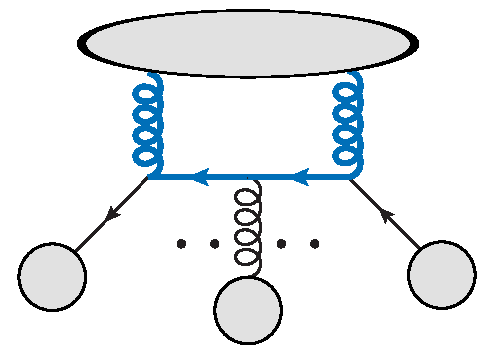
\includegraphics[width=0.35\textwidth]{figures/protochain}
  \caption{A schematic subdiagram of a fermion line entering and
    leaving the loop giving rise to a generic spinor string. The grey circles represent tree-like
    contributions and lines carrying loop momentum are thick and colored (blue).}
  \label{fig:spinchain}
\end{figure}
When fermion lines enter (and leave) the loop, they
contribute generic strings of Dirac matrices to Feynman diagrams
(Fig.~\ref{fig:spinchain}). The source of Dirac matrices contributing
to the partial trace over $\dtt$ in Eq.~\eqref{eq:tr1l} is twofold. Vertices of quarks coupled to
gluons carrying loop momentum are proportional to $\gm{\mu}{D_s}{\dt}$
and quark propagators carrying loop momentum can be written, using relations \eqref{eq:loopmom}, as
\begin{align}\label{eq:qprop}
 \prescript{(\dt)}{}{ S_{\text{q}}(\ell_{[D]})}&=
 \frac{i}{\ell^2_{[D]}-m^2}\left(\ell^{\phantom{\mu}}_{[D]\,\mu}\gm{\mu}{D_s}{\dt}+m\cdot\prescript{(\dt)}{}{\mathbb{1}_{\phantom{\mu}}^{\phantom{\mu}}}\right)\\
&= 
  \frac{i}{\ell^2_{[4]}-\mu^2-m^2}\left( \prescript{(\dt)}{}{\slashed{\ell}_{[4]}} +m\cdot\prescript{(\dt)}{}{\mathbb{1}} + \mu\,\gmt{4}{\dt} \right).
\end{align}
The only non-trivial contribution of Eq.~\eqref{eq:qprop} comes from $\mu\gmt{4}{\dt}$,
since the two other terms are proportional to a
unit matrix in the $\dtt$-space. For the tensorial split-up of the matrices $\gmt{4}{\dt}$ in quark propagators, we adapt Eq.~\eqref{eq:highgamma} for later convenience to  
\begin{align}\label{eq:prohg}
\gmt{4}{\dt} = \gtw{4}{(\dtt)} \otimes  {\g5} =  \left(-i\gtw{4}{(\dtt)} \right) \otimes  (i{\g5}),
\end{align}
such that $(-i\gtw{4}{})\cdot(-i\gtw{4}{})=1$.

A generic spinor string
$T^{\mu\nu}_{[D_s]}$, with indices coupled to $D_s$-dimensional
gluons in the loop left uncontracted, is according to the prescription
we found in the previous Section~\ref{sec:olmetrace}, see Eq.~\eqref{eq:tr1l}, of the form
\begin{equation}\label{eq:protochain}
  T^{\mu\nu}_{[D_s]} = \tr[\dtt]{M^{\mu\nu}_n},
\end{equation}
with 
\begin{equation}
  M^{\mu\nu}_n =  \langle p_1, i_1 |\cdots \gm{\mu}{D_s}{\dt} \left( \prod_{k=1}^{n}\gm{4}{D_s}{\dt} \cdots \right) \gm{\nu}{D_s}{\dt}\cdots | p_2, i_2 \rangle.
\end{equation}
The dots $\cdots$ represent any number of $\dt$-dimensional
gamma matrices from vertices and propagators that contribute only a unit matrix to the partial trace over $\dtt$. The number of insertions
of $\gmt{4}{\dt}$ from quark
propagators is denoted by $n$, see Eq.~\eqref{eq:qprop}.

The partial trace of $M^{\mu\nu}_n$ over $\dtt$ in
Eq.~\eqref{eq:protochain} can be evaluated explicitly using the tensor
product structure of gamma matrices shown in Eqs.~\eqref{eq:fourgamma}
and \eqref{eq:highgamma}. It is only non-vanishing
for an even number of $\gtw{\mu}{}$ matrices in the trace, as shown in
Eq.~\eqref{eq:tracehddodd}. We distinguish four cases depending on
whether the matrices $\gtw{\mu}{}$ in the partial trace originate in insertions from the
quark propagator or in vertex couplings to the higher-dimensional
scalar components of a $D_s$-dimensional gluon. We start with a restriction of the
open indices of Eq.~\eqref{eq:protochain} to $\mu,\nu \leq 3$, corresponding to a coupling of the
spinor string to two ``massive'' gluons, which leads to 
\begin{subequations}
\begin{align}
    T^{\mu\nu}_{[D_s]} = \tr[\dtt]{M^{\mu\nu}_n} &=\trf[(-i\gtw{4}{})^n] ~ \big(\cdots \gamma^{\mu}\cdots\gamma^{\nu}\cdots\big), &&\mu,\nu \leq 3,\\\label{eq:mgcont}
&= \dtt  ~ \big(\cdots \gamma^{\mu}\cdots\gamma^{\nu}\cdots\big), &&n\text{ even},
\end{align}
\end{subequations}
which is only non-vanishing for an even number $n$ of $\gmt{4}{\dt}$
insertions from quark propagators. We used Eqs.~\eqref{eq:fourgamma}
and \eqref{eq:prohg} such that $(-i\gtw{4}{})\cdot(-i\gtw{4}{})=1$. The expression in parentheses denotes the remaining
four-dimensional part of the spinor string. We explicitly show the four-dimensional
matrices at the two uncontracted vertices. The four-dimensional parts
$i\g5$ of the insertions from quark
propagators are not explicitly shown and accounted for in the quark propagator. We proceed in the same manner with the
remaining cases. A restriction of both open indices to $\mu,\nu \geq
4$, corresponding to a coupling to two scalars, leads to
\begin{subequations}
\begin{align}
    T^{\mu\nu}_{[D_s]} = \tr[\dtt]{M^{\mu\nu}_n} &=\trf[\gtw{\mu}{}(-i\gtw{4}{})^n\gtw{\nu}{}] ~ \big(\cdots \g5\cdots\g5\cdots\big), &&\mu,\nu \geq 4,\\\label{eq:twosccont}
&= \dtt ~ \big(\cdots \g5\cdots\g5\cdots\big) ~ g_{[D_s-4]}^{\mu\nu}, &&n\text{ even},
\end{align}
\end{subequations}
which is again only non-vanishing for even powers $n$ of $\gmt{4}{\dt}$
insertions from quark propagators. We used the same relations as for
the previous case and additionally Eq.~\eqref{eq:nontrivtrace} to evaluate the
non-trivial trace over $\dtt$. Lastly, we treat the two related cases
of $\mu \leq 3, \nu \geq 4$ and vice versa, corresponding to the
coupling of a spinor string to both a ``massive'' gluon and a
scalar. The expression for the spinor string is given by
\begin{subequations}
\begin{align}
    T^{\mu\nu}_{[D_s]} = \tr[\dtt]{M^{\mu\nu}_n} &=
\begin{cases}
\trf[\gtw{\mu}{}(-i\gtw{4}{})^n] ~  \big(\cdots \g5\cdots\gamma^{\nu}\cdots\big)\qquad\mu \geq 4, \nu \leq 3,\\
\trf[(-i\gtw{4}{})^n\gtw{\nu}{}] ~ \big(\cdots
\gamma^{\mu}\cdots\g5\cdots\big)\qquad \mu \leq 3, \nu \geq 4,
\end{cases}\\\label{eq:mixcont}
&=-i\dtt 
\begin{cases}
  \big(\cdots
\g5\cdots\gamma^{\nu}\cdots\big) ~ g_{[D_s-4]}^{\mu 4 },\\
\big(\cdots \gamma^{\mu}\cdots\g5\cdots\big) ~ g_{[D_s-4]}^{\nu 4 },
\end{cases}n\text{ odd},
\end{align}
\end{subequations}
where we used the same relations as above to evaluate the partial
trace. 

The resulting expressions of Eqs.~\eqref{eq:mgcont}, \eqref{eq:twosccont} and \eqref{eq:mixcont} are contracted
with the remainder of the loop diagram $D^{\mu\nu}_{[D_s]}$, which we
write as $( \{\cdots\}_{[4]\,\mu\nu} +
\{\cdots\}g^{\phantom{\mu}}_{[D_s-5]\,\mu\nu} )$. In this relation, we used the decoupling
of scalars and ``massive'' gluons described around Eq.~\eqref{eq:axgaugprop}. $\{\cdots\}_{[4]\,\mu\nu}$ is a four-dimensional tensor
denoting a contribution from the latter and
$\{\cdots\}g^{\phantom{\mu}}_{[D_s-5]\,\mu\nu}$ is a tensor
denoting the scalar contribution. For a
single fermion line entering the loop, we have a single spinor string
$T^{\mu\nu}_{[D_s]}$ and the contraction is of the form
\begin{equation} \label{eq:contr1}
  T^{\mu\nu}_{[D_s]} D^{\phantom{\mu}}_{[D_s]\,\mu\nu} = 
  T^{\mu\nu}_{[D_s]}\left( \{\cdots\}_{[4]\,\mu\nu} + \{\cdots\}g^{\phantom{\mu}}_{[D_s-5]\,\mu\nu} \right)= 
  \dtt\left( d_{\text{gl}} + (D_s-5)\,d_{\text{sc}}  \right),
\end{equation}
where $d_{\text{gl}}$ is a diagram with all $D_s$ dimensional gluons
replaced by ``massive'' gluons and $d_{\text{sc}}$ a diagram with all
$D_s$ dimensional gluons replaced with scalars. In the second equality
we used Eqs.~\eqref{eq:mgcont}, \eqref{eq:twosccont} and
\eqref{eq:mixcont} and the property of the metric tensor
\begin{equation} \label{eq:metrconr}
  g^{\mu\nu}_{[D_s-4]}g_{[D_s-5]\,\nu\mu}^{\phantom{\mu}}=g^\mu_{\mu\,[D_s-5]}=(D_s-5).
\end{equation}

For loop diagrams with multiple quark lines entering the loop, the
split-up of $D_s$-dimensional gluons leads to mixed diagrams with both
``massive'' gluons and scalars coupling to the same spinor string that have to be considered in general. However, it turns out that the contraction of a fermion line with a ``massive'' gluon on one side and
with a scalar on the other side vanishes. In this situation, the cases
of Eq.~\eqref{eq:mixcont} are used, and the contraction with both a
``massive'' gluon and a scalar propagator leads to:
\begin{equation}
  g_{[D_s-5]}^{\mu \nu  } g_{[D_s-4]\, \nu 4}^{\phantom{\mu}} = g_{[D_s-5]}^{\mu 4} = 0.
\end{equation}
Therefore, also for multiple fermion lines in the loop the diagrams in which all $D_s$-dimensional gluons are replaced by
``massive'' gluons and those with all $D_s$-dimensional
gluons replaced by scalars can be treated independently. Diagrams with scalars
in the loop pick up a factor of $(D_s-5)$ from contractions across
multiple lines, see Eq~\eqref{eq:metrconr}. The additional prefactor
$\dtt$ from the partial trace over each spinor string in
Eqs.~\eqref{eq:mgcont}, \eqref{eq:twosccont} and \eqref{eq:mixcont} cancels with that
in Eq.~\eqref{eq:tr1l}.

Summing up, we found that all diagrams under consideration exhibit the same dimensional dependence and respect the decoupling of ``massive'' gluons and scalars.
Hence a one-loop amplitude with any number of external quark pairs\footnote{For now we exclude diagrams with closed fermion loops,
  which we will discuss later.} can be written in arbitrary $D_s$ as
\begin{equation} 
  \mathcal{A}^{[D_s]}_{\text{ext}\in S_{[4]}} =\Big( \mathcal{A}_{\text{gl}} + (D_s-5)~\mathcal{A}_{\text{sc}}\Big),
  \label{eq:ddependence}
\end{equation}
where $\mathcal{A}_{\text{gl}}$ is a sum of diagrams with ``massive''
gluons and $\mathcal{A}_{\text{sc}}$ is a sum of diagrams with
scalars in the loop. Both $\mathcal{A}_{\text{gl}}$ and
$\mathcal{A}_{\text{sc}}$ are defined in terms of four-dimensional
objects in addition with the requirement of only even number of $(D_s-4)$-dimensional loop momenta insertions from the quark propagator Eq.~\eqref{eq:qprop} on \emph{each}
fermion line. The latter is in general impossible to satisfy with \emph{only} four-dimensional representations of the Dirac
algebra. We provide further details of a numerical computation of
$\mathcal{A}_{\text{gl}}$ and $\mathcal{A}_{\text{sc}}$ in Sec.~\ref{sec:impl-deta}.

Once the full dimensional dependence is established by Eq.~\eqref{eq:ddependence}, we can use it to \emph{define}
an amplitude for continuous $D_s$. An FDH amplitude is obtained by setting $D_s=4$:
\begin{equation} \label{eq:decgsc}
  \mathcal{A}^{\text{FDH}} = \mathcal{A}_{\text{gl}} - \mathcal{A}_{\text{sc}}.
\end{equation}
The connection to the method of dimensional reconstruction \cite{Giele:2008ve} can be made clear by using Eq.~\eqref{eq:ddependence} with the following
\begin{equation}
  \mathcal{A}^{\text{FDH}} = 2\mathcal{A}^{[6]}_{\text{ext}\in S_{[4]}} - \mathcal{A}^{[8]}_{\text{ext}\in S_{[4]}} = \mathcal{A}^{[6]}_{\text{ext}\in S_{[4]}} - 2{\mathcal{A}}_{\text{sc}},
\end{equation}
which is valid for all QCD one-loop amplitudes. We used
Eq.~\eqref{eq:ddependence} and the above can be
further compressed to Eq.~\eqref{eq:decgsc}.

It remains to analyze diagrams with a closed fermion loop. For those, no
$D_s$-dimensional vector index contractions appear and the only
possible dimensional dependence is an additional total factor of
$\dtt$ from the loop trace. To see this in detail, we analyze a generic
contribution to the $D_s$-dimensional loop trace which is of the form
\begin{align}
\begin{split}
T^{\mu_1\cdots \mu_n}_{n_f\ [D_s]}  &=
\tr[\dtt]{\left(-i\gtw{4}{(\dtt)}\right)\cdots\left(-i\gtw{4}{(\dtt)}\right)}\tr[4]{\gamma^{\mu_1}\cdots
\gamma^{\mu_n}}\\
&=\dtt \tr[4]{\gamma^{\mu_1}\cdots
\gamma^{\mu_n}}.
\end{split}
\end{align}
Both traces above are only non-vanishing for even
powers of $\gtw{4}{(\dtt)}$ from propagator insertions. Odd numbers of higher-dimensional loop momenta insertions
  lead to vanishing traces over odd numbers of $\g5$ in the
  four-dimensional trace. The requirement to have only even powers of
$\gtw{4}{(\dtt)}$ insertions can thus be satisfied with a purely
four-dimensional calculation and a four-dimensional quark propagator
carrying a dependence on $\mu$ (cf.~Sec.~\ref{sec:impl-deta}). We get the simple relation
\begin{equation} \label{eq:nfdecomp}
  \mathcal{A}^{\text{FDH}}_{\text{nf}} =
  \frac{1}{\dtt}{\mathcal{A}}^{[D_s]}_{\text{nf}} = {\mathcal{A}}^{[4]}_{\text{nf}} .
\end{equation}
We implemented the approach discussed in this section in the
\BlackHat~library. A detailed verification of NLO QCD virtual matrix
elements computed with the above prescription is performed in Chapter
\ref{chap:wbb_validation}. We do so by comparing all QCD
processes with up to 7 partons as well
as those with the associated emission of a $W^{\pm}$
boson\footnote{Chiral couplings can be incorporated using the 't Hooft-Veltman
  prescription, see Section~\ref{subsec:g5}.
} 
with publicly available tools.


%%%%%%%%%%%%%%%%%%%%%%%%%%%%%%%%%%%%%%%%%%%%%%%%%%%
%%%%%%%%%%%%%%%%%%%%%%%%%%%%%%%%%%%%%%%%%%%%%%%%%%%


\section{Remarks on the FDF Scheme}
\label{sec:fdf}
In this section, we discuss the connection of our prescription
formulated in the previous section to the
recently proposed four-dimensional (re-)formulation (FDF) of FDH \cite{Fazio:2014xea}.
It provides a computational prescription in four dimensions together with
selection rules, which have to be evaluated at the level of Feynman
diagrams\footnote{The evaluation of the selection rules has to be done
  only once for a given process, comparable to the color algebra.}. The
scheme is defined with the additional requirement to
remove odd powers of $\mu$ from the integrand. For testing purposes, we have implemented the FDF method in the context of our numerical unitarity calculation. We find that for amplitudes with gluons and a single quark line, the application of
the FDF prescription is equivalent to Eq.~\eqref{eq:decgsc}, which can
be seen by computing the relevant selection rule factors.


However, for processes involving multiple quark lines, the requirement to remove
odd powers of $\mu$ is in general not sufficient to circumvent the obstruction discussed below
Eq.~\eqref{eq:ddependence}.
\begin{figure}%{L}{0.5\textwidth}
  \centering
  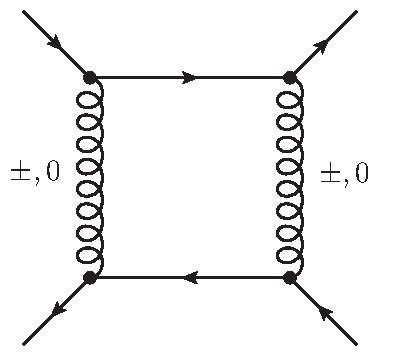
\includegraphics[clip,width=0.3\textwidth]{figures/mu2_draft.pdf}
  \caption{Diagram for the exchange of two ``massive''
    gluons between two quark lines in the FDF. It contains terms that
  are proportional to $\mu^2$, which vanish in the FDH scheme. }
  \label{fig:mu2ex}
\end{figure}
As an example we consider the evaluation of the diagram in Fig.~\ref{fig:mu2ex}, that
is the exchange of two ``massive'' gluons (cf.~Sec.~\ref{sec:glue-axial}) between two quark lines. If both
quark lines are massive%
%\footnote{Note that this type of term vanishes as soon as one of the quark lines is massless, cf.~Eq.~\eqref{eq:masslesssim}.}
, there is a non-vanishing contribution of the form
\begin{align}\label{eq:probfdf}
  \langle p_2|\gamma^\mu (i\mu\g5) \gamma^\nu  |p_1\rangle   \langle
  p_4|\gamma^\rho(i\mu\g5) \gamma^\sigma  |p_3\rangle
  D^{\text{mg}}_{\mu\sigma} D^{\text{mg}}_{\nu\rho} \sim \mu^2 \cdots.
\end{align}
Terms with odd numbers of $\mu$ insertions, that combine to even powers
of $\mu$ across multiple lines, generically appear in FDF with two
or more massive quark lines.
In FDH however, these terms are removed at each line by the partial traces over
$\dtt$. They thus constitute a genuine difference between the FDF and
the FDH scheme.

In the following, we propose a modification of the FDF prescription to
correctly reproduce one-loop FDH amplitudes with multiple (massive)
quark lines. In the FDF, one performs the substitutions 
\begin{align}\label{eq:fdfrep}
  g^{\mu\nu}_{[D_s-4]} &\rightarrow G^{AB}, &
  \gamma^\mu_{[D_s-4]}&\rightarrow \g5 \Gamma^A,  &
  \ell^\mu_{[D_s-4]}&\rightarrow i\mu Q^A,
\end{align}
where symbols $\Gamma^A$ do not have a finite-dimensional representation.
The FDF is then
based on the formulation of selection rules for the objects $G^{AB}$,
$\Gamma^A$ and $Q^A$. Amongst them, the replacements of
Eq.~\eqref{eq:fdfrep} lead to the selection rule
\begin{align}\label{eq:wrongsr}
  \slashed{\ell}_{[D_s-4]}  \slashed{\ell}_{[D_s-4]} = - \mu^2
  Q^A\Gamma^AQ^B\Gamma^B &= -\mu^2 & &\rightarrow& Q^A\Gamma^A &=1.
\end{align}
However the last transition is ad hoc, since the above equation allows
more solutions in general. For example,
one can easily find a non-unit matrix that squares to a
unit matrix.
The corrected selection rule drawn from Eq.~\eqref{eq:wrongsr} is thus
\begin{align}\label{eq:nsr}
  Q^A\Gamma^AQ^B\Gamma^B &=1.
\end{align}

We propose to replace the selection rule in Eq.~\eqref{eq:wrongsr} with
that in Eq.~\eqref{eq:nsr}. Together with the rules to
contract indices across different quark lines equivalent to
Eqs.~\eqref{eq:mgcont}, \eqref{eq:twosccont} and \eqref{eq:mixcont}, the FDF becomes a valid (re-)formulation of
FDH applicable to amplitudes with multiple quark lines.
An implementation of the FDF is thus equivalent to the one described in the Section~\ref{sec:impl-deta}.


\section{Implementation Details}
\label{sec:impl-deta}
In this section, we describe details required for a numerical implementation of the
prescription that we presented in Sec.~\ref{sec:gener-spin-chains}, see
Eq.~\eqref{eq:decgsc} and Eq.~\eqref{eq:nfdecomp}. It allows to compute one-loop QCD amplitudes involving multiple (massive)
quark lines regularized
in the FDH scheme in a compact way.

An FDH amplitude is given by the difference
of an amplitude with all $D_s$ dimensional gluons replaced by a four-dimensional
``massive'' gluon in the loop and one
with scalar particles in the loop, see Eq.~\eqref{eq:decgsc}. These amplitudes are defined in
terms of four-dimensional objects. Additionally, the requirement of even numbers of $(D_s-4)$-dimensional loop momentum insertions
from quark propagators on each fermion line has to be enforced. We propose to
keep track of the number of $(D_s-4)$ insertions from quark
propagators to enforce this requirement. One way to achieve this
numerically is to use a double copy of fermionic states and vertices
and to adapt the $\mu$-dependent piece of the propagator to switch
between upper and lower components, see Feynman rules in Table \ref{tab:fr}.\footnote{This
  is related to a calculation in $D_s=6$ dimensions but
  differs in the treatment of external states.} For external and
  internal fermionic particles, the states are constructed as described in
  Sec.~\ref{sec:fermionic-states} with $D_s=6$. For external particles, only the states
with \dttindex{} $j=0$ are considered, which projects out terms with even numbers
of insertions of $(D_s-4)$-dimensional loop momenta. One can equally
think of this as keeping track of even powers of $\mu$.


An additional simplification can be
exploited for massless quark lines, since odd numbers of $\g5$ matrices in a massless spinor
chain vanish
\begin{align}\label{eq:masslesssim}
  \langle p_1,i_1|\cdots \g5 \cdots | p_2,i_2\rangle &= 0, &
  p_1^2&=p_2^2=0,
\end{align}
and the requirement to have only even numbers of $(D_s-4)$-dimensional loop momentum insertions is automatically
fulfilled. In this situation, it suffices to compute with a $D_s=4$
dimensional representation of gamma matrices in vertices and the quark propagator 
\begin{align}\label{eq:4dquark}
\prescript{(4)}{}{ S_{\text{q}}(\ell_{[D]})}= \frac{i\left(\prescript{(4)}{}{\slashed{\ell}_{[4]}} + i\mu \g5 + m\right)}{\ell_{[4]}^2-\mu^2-m^2},
\end{align}
on massless fermion lines. A similar simplification applies to closed fermion
  loops. Odd numbers of higher-dimensional loop momenta insertions
  lead to vanishing traces over odd numbers of $\g5$. Consequently,
  the requirement of having even numbers of insertions is always
  fulfilled and it
  suffices to compute in four-dimensions with the quark propagator of
  Eq.~\eqref{eq:4dquark}. To illustrate the prescription, we show in
Eqs.~\eqref{eq:pics}-\eqref{eq:picsf} the schematic computation of FDH amplitudes in terms of ``massive'' gluon
  and scalar amplitudes with even numbers of $(D_s-4)$-dimensional loop
  momenta insertions. We show the examples of gluon and closed fermion
  diagrams, as well as those with (multiple) quark lines entering the loop. The dimension $\dt$ of fermion states in the loop is written between parentheses. 

In summary, in this chapter we provide a compact algorithm for the
computation of NLO QCD amplitudes regularized in FDH. We find a simple
and computationally efficient decomposition of
amplitudes by particle content in the loop. $D_s$ dimensional gluons
circulating in the loop are replaced by a ``massive'' four-dimensional
gluon as well as a colored scalar. In a numerical
implementation, we propose to keep track of even powers of $\mu$ by
using a $D_s=6$-dimensional representation of the Dirac algebra for
vertices and propagators. Our central result is a generalization of
the previously known decomposition for gluons \cite{Bern:1994cg} to the full QCD
spectrum, and is in particular valid for multiple massive quark
lines. We furthermore clarify the connection between dimensional
reconstruction methods and the FDF \cite{Fazio:2014xea} and find equivalence
for gluon amplitudes and those with a single quark line. For
multiple quark lines however, the FDF contains terms that constitute a
genuine difference with respect to FDH. We provide an adaption of the selection
rules and thereby make the FDF applicable to amplitudes with multiple
quark lines.




\begin{table}[]
\centering
\caption{Color-ordered QCD Feynman rules for the computation of
  FDH one-loop amplitudes. Shown are the rules for ``massive'' gluons
  and scalars in the loop. The requirement to have even
  numbers of insertions of higher-dimensional loop momentum along each
fermion line is enforced by construction.}
\label{tab:fr}
\begin{tabular}{l}
\begin{tabularx}{\textwidth}{ll}
    \noalign{\vskip 2.5mm}
    \hline\hline
    \noalign{\vskip 2.5mm}
    \textbf{Propagators}\\
    \noalign{\vskip 2mm}
    \hline
    \noalign{\vskip 4mm}
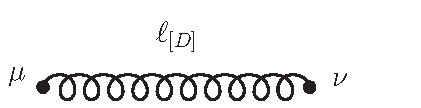
\includegraphics[clip,width=0.2\textwidth]{figures/gp}
&$\displaystyle =\frac{i}{\ell_{[4]}^2-\mu^2}\left[-g^{\mu\nu}_{[4]}+
  \frac{\ell^\mu_{[4]}\ell^\nu_{[4]}}{\mu^2}\right]$\\

\includegraphics[clip,width=0.15\textwidth]{figures/qp} &
$\displaystyle  = \frac{i}{\ell_{[4]}^2-\mu^2-m^2} \left[\prescript{(2)}{}{\mathbb{1}}\otimes
  \left(\prescript{(4)}{}{\slashed{\ell}_{[4]}} +
     m\,\prescript{(4)}{}{\mathbb{1}}\right)  + \pmqty{0 & 1 \\ 1 & 0}
   \otimes i\mu\g5\right] $\\

\includegraphics[clip,width=0.15\textwidth]{figures/sp} &
$\displaystyle  = \frac{-i}{\ell^2_{[4]}-\mu^2} $\\
    \noalign{\vskip 2.5mm}
    \hline
    \noalign{\vskip 2.5mm}
    \textbf{Vertices}\\
    \noalign{\vskip 2mm}
    \hline
    \noalign{\vskip 4mm}
\raisebox{-.4\height}{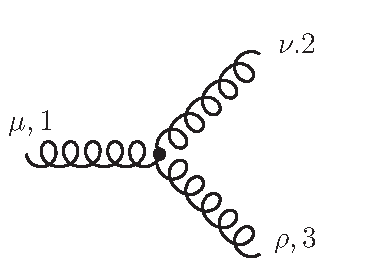
\includegraphics[clip,width=0.2\textwidth]{figures/gggv}} &
$\displaystyle  = \frac{i}{\sqrt{2}}\left[g_{[4]}^{\mu\nu}(p_{1\,[4]}-p_{2\,[4]})^\rho+g_{[4]}^{\nu\rho}(p_{2\,[4]}-p_{3\,[4]})^\mu+g_{[4]}^{\rho\mu}(p_{3\,[4]}-p_{1\,[4]})^\nu\right]
$\\
\raisebox{-.4\height}{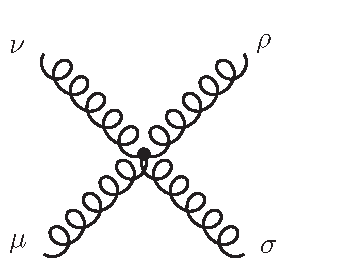
\includegraphics[clip,width=0.2\textwidth]{figures/gggg}} &
$\displaystyle  = ig_{[4]}^{\mu\rho}g_{[4]}^{\nu\sigma} -
\frac{i}{2}\left[g_{[4]}^{\mu\nu}g_{[4]}^{\rho\sigma}+g_{[4]}^{\mu\sigma}g_{[4]}^{\nu\rho}\right]
$
\end{tabularx}\\
\begin{tabularx}{\textwidth}{llll}
\raisebox{-.4\height}{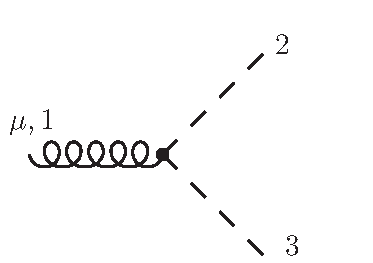
\includegraphics[clip,width=0.2\textwidth]{figures/ssg}} &
$\displaystyle  =  \frac{i}{\sqrt{2}}  (p_{2\,[4]}-p_{3\,[4]})^\mu$&
\raisebox{-.4\height}{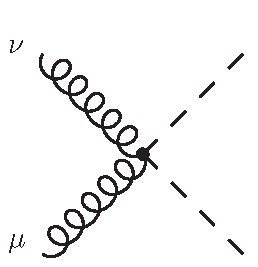
\includegraphics[clip,width=0.15\textwidth]{figures/ssgg}} &
$\displaystyle  =  - \frac{i}{2}   g_{[4]}^{\mu\nu}$\\
\raisebox{-.4\height}{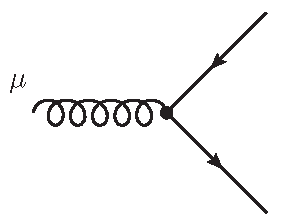
\includegraphics[clip,width=0.15\textwidth]{figures/qqg}} &
$\displaystyle  = \frac{i}{\sqrt{2}} \prescript{(2)}{}{\mathbb{1}}
\otimes \gamma^\mu $&
\raisebox{-.4\height}{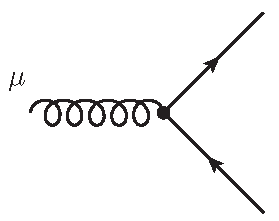
\includegraphics[clip,width=0.15\textwidth]{figures/qqg2}} &
$\displaystyle  = -\frac{i}{\sqrt{2}} \prescript{(2)}{}{\mathbb{1}}
\otimes \gamma^\mu $\\
\raisebox{-.4\height}{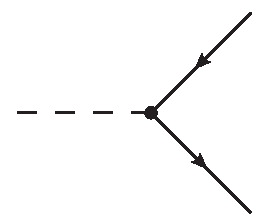
\includegraphics[clip,width=0.15\textwidth]{figures/qqs}} &
$\displaystyle  = \frac{i}{\sqrt{2}} \prescript{(2)}{}{\mathbb{1}}\otimes\g5$&
\raisebox{-.4\height}{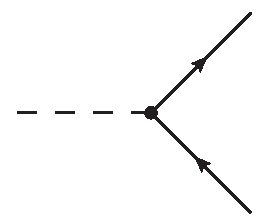
\includegraphics[clip,width=0.15\textwidth]{figures/qqs2}} &
$\displaystyle  = -\frac{i}{\sqrt{2}}\prescript{(2)}{}{\mathbb{1}}
\otimes\g5$\\
    \noalign{\vskip 4mm}
    \hline
    \noalign{\vskip 2.5mm}
    \textbf{Outgoing Fields}\\
    \noalign{\vskip 2mm}
    \hline
    \noalign{\vskip 3mm}
\raisebox{-.1\height}{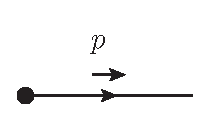
\includegraphics[clip,width=0.15\textwidth]{figures/wfq}} &
$\displaystyle  = \pmqty{\prescript{(4)}{}{\bar{u}(p)},&0}$&
\raisebox{-.1\height}{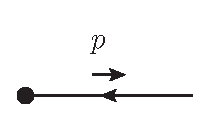
\includegraphics[clip,width=0.15\textwidth]{figures/wfqb}} &
$\displaystyle  = \pmqty{\prescript{(4)}{}{v(p)} \\ 0}$\\
    \noalign{\vskip 4mm}    
\hline\hline
\end{tabularx}
\end{tabular}
\end{table}


\begin{align}
\label{eq:pics}
  \vcenter{\hbox{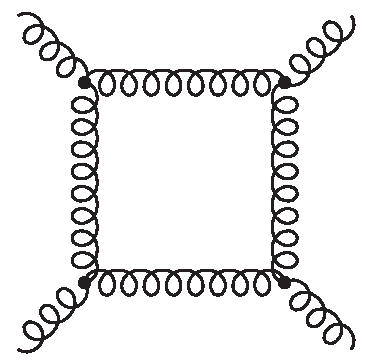
\includegraphics[clip,width=0.2\textwidth]{figures/0q}}}
  &\xrightarrow{D_s\rightarrow 4}   \vcenter{\hbox{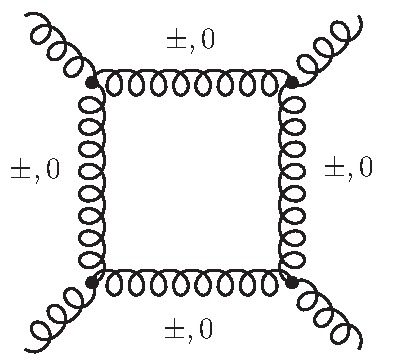
\includegraphics[clip,width=0.221\textwidth]{figures/0q_glue}}} -   \vcenter{\hbox{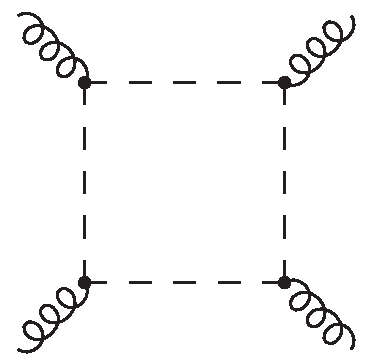
\includegraphics[clip,width=0.2\textwidth]{figures/0q_sc}}}\\
  \vcenter{\hbox{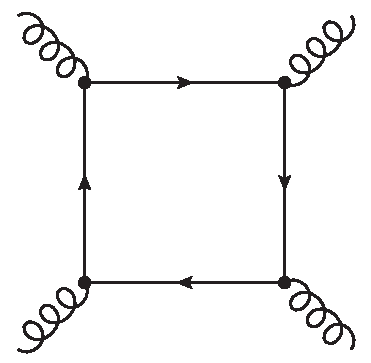
\includegraphics[clip,width=0.2\textwidth]{figures/0q2}}}
 &\xrightarrow{D_s\rightarrow 4}   \vcenter{\hbox{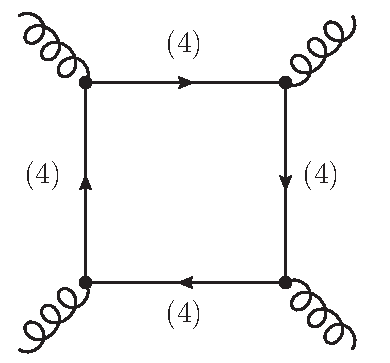
\includegraphics[clip,width=0.2\textwidth]{figures/0q_q}}}\\
  \vcenter{\hbox{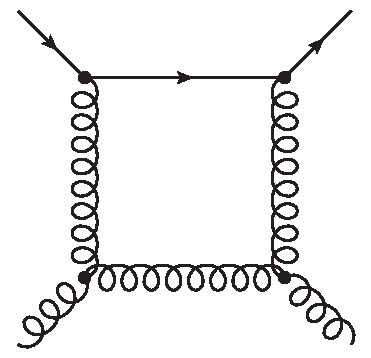
\includegraphics[clip,width=0.2\textwidth]{figures/1q}}}
  &\xrightarrow{D_s\rightarrow 4}
  \vcenter{\hbox{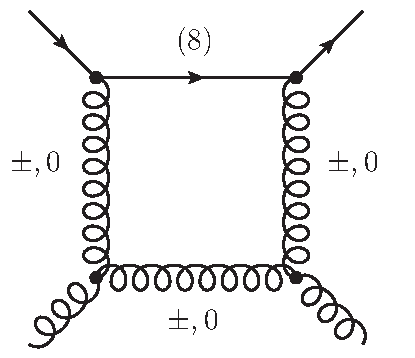
\includegraphics[clip,width=0.221\textwidth]{figures/1q_glue}}}
  -
  \vcenter{\hbox{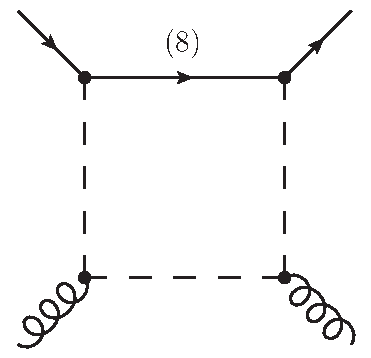
\includegraphics[clip,width=0.2\textwidth]{figures/1q_sc}}}\\
\label{eq:picsf}
  \vcenter{\hbox{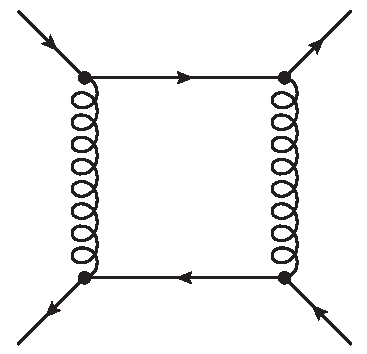
\includegraphics[clip,width=0.2\textwidth]{figures/2q}}}
 & \xrightarrow{D_s\rightarrow 4}     \vcenter{\hbox{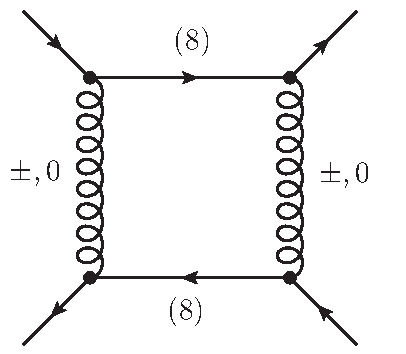
\includegraphics[clip,width=0.221\textwidth]{figures/2q_glue}}} -   \vcenter{\hbox{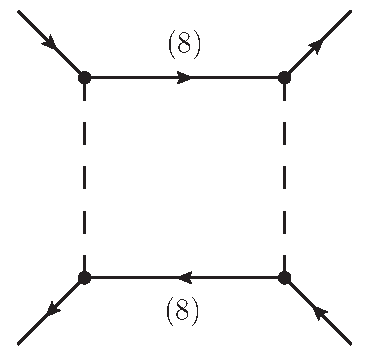
\includegraphics[clip,width=0.2\textwidth]{figures/2q_sc}}}
\end{align}

%\clearpage


%%%%%%%%%%%%%%%%%%%%%%%%%%%%%%%%%%%%%%%%%%%%%%%%%%%
%%%%%%%%%%%%%%%%%%%%%%%%%%%%%%%%%%%%%%%%%%%%%%%%%%%
%%%%%%%%%%%%%%%%%%%%%%%%%%%%%%%%%%%%%%%%%%%%%%%%%%%


%%%%%%%%%%%%%%%%%%%%%%%%%%%%%%%%%%%%%%%%%%%%%%%%%%%
%%%%%%%%%%%%%%%%%%%%%%%%%%%%%%%%%%%%%%%%%%%%%%%%%%%




%%% Local Variables: 
%%% mode: latex
%%% TeX-master: "../diss"
%%% End: 
